\documentclass[11pt]{article}
\usepackage[margin=0.82in]{geometry}
\usepackage{amsmath,amssymb,amsthm,mathtools}
\usepackage{graphicx}
\usepackage{microtype}
\usepackage[hidelinks]{hyperref}
\usepackage{xcolor}

\newtheorem{theorem}{Theorem}
\newtheorem{lemma}{Lemma}
\newcommand{\Pp}{\mathbb P}
\newcommand{\E}{\mathbb E}
\newcommand{\ellf}{\ell}
\newcommand{\Tp}[1]{T_{#1}}
\newcommand{\asym}{\asymp}

\title{The logarithmic loss in the bounded-support tail estimate is sharp}
\author{Candidate full solution for arXiv:1706.07539}
\date{9 August 2026}

\begin{document}
\maketitle

\begin{center}
\fbox{\parbox{0.92\linewidth}{
\textbf{Status.} Candidate full solution, subject to human verification.  The
answer to the open question following (3.19b) is \(\boxed{\gamma+1}\).  The
published upper estimate already has this exponent; the construction below
shows that no smaller exponent works under the paper's hypotheses, even when
the operator is positive, linear, and contractive on every \(L^p\),
\(1\le p\le b\).
}}
\end{center}

\begin{abstract}
Ostrovsky and Sirota prove that a tail bound
\(T_f(y)\le y^{-b}(\log y)^\gamma L(\log y)\) is transferred by an operator of
equal-power type to a bound with logarithmic exponent \(\gamma+1\), and ask
for the optimal replacement of that exponent.  We build a positive linear
\(L^p\)-contraction which, on sparse atomic blocks, maps a function having the
source tail to an image whose tail attains the \(\gamma+1\) power along an
unbounded sequence.  Thus the one-logarithm loss is unavoidable in the stated
operator class.
\end{abstract}

\section{Source question}

The source is E. Ostrovsky and L. Sirota, \emph{Maximal and other operators in
exponential Orlicz and Grand Lebesgue Spaces}, arXiv:1706.07539 (2017)
\cite{OS}.  In Example 3.2, pp.~17--18, they fix \(b>1\), \(\gamma>-1\), and
a positive slowly varying function \(L\), assume
\[
 \Tp f(y)\le y^{-b}(\log y)^\gamma L(\log y),\qquad y\ge e,
\]
and derive
\[
 \Tp g(y)\le C y^{-b}(\log y)^{\gamma+1}L(\log y).
\]
Immediately after (3.19b), they ask: ``what is the ultimate value instead
\(\gamma+1\) in the last estimate?''

\begin{figure}[p]
\centering

\includegraphics[width=0.92\textwidth]{figures/open_problem_crop_page17.png}
\caption{Source paper, p.~17: assumptions (3.18) and upper estimate (3.19a).}
\end{figure}

\begin{figure}[p]
\centering
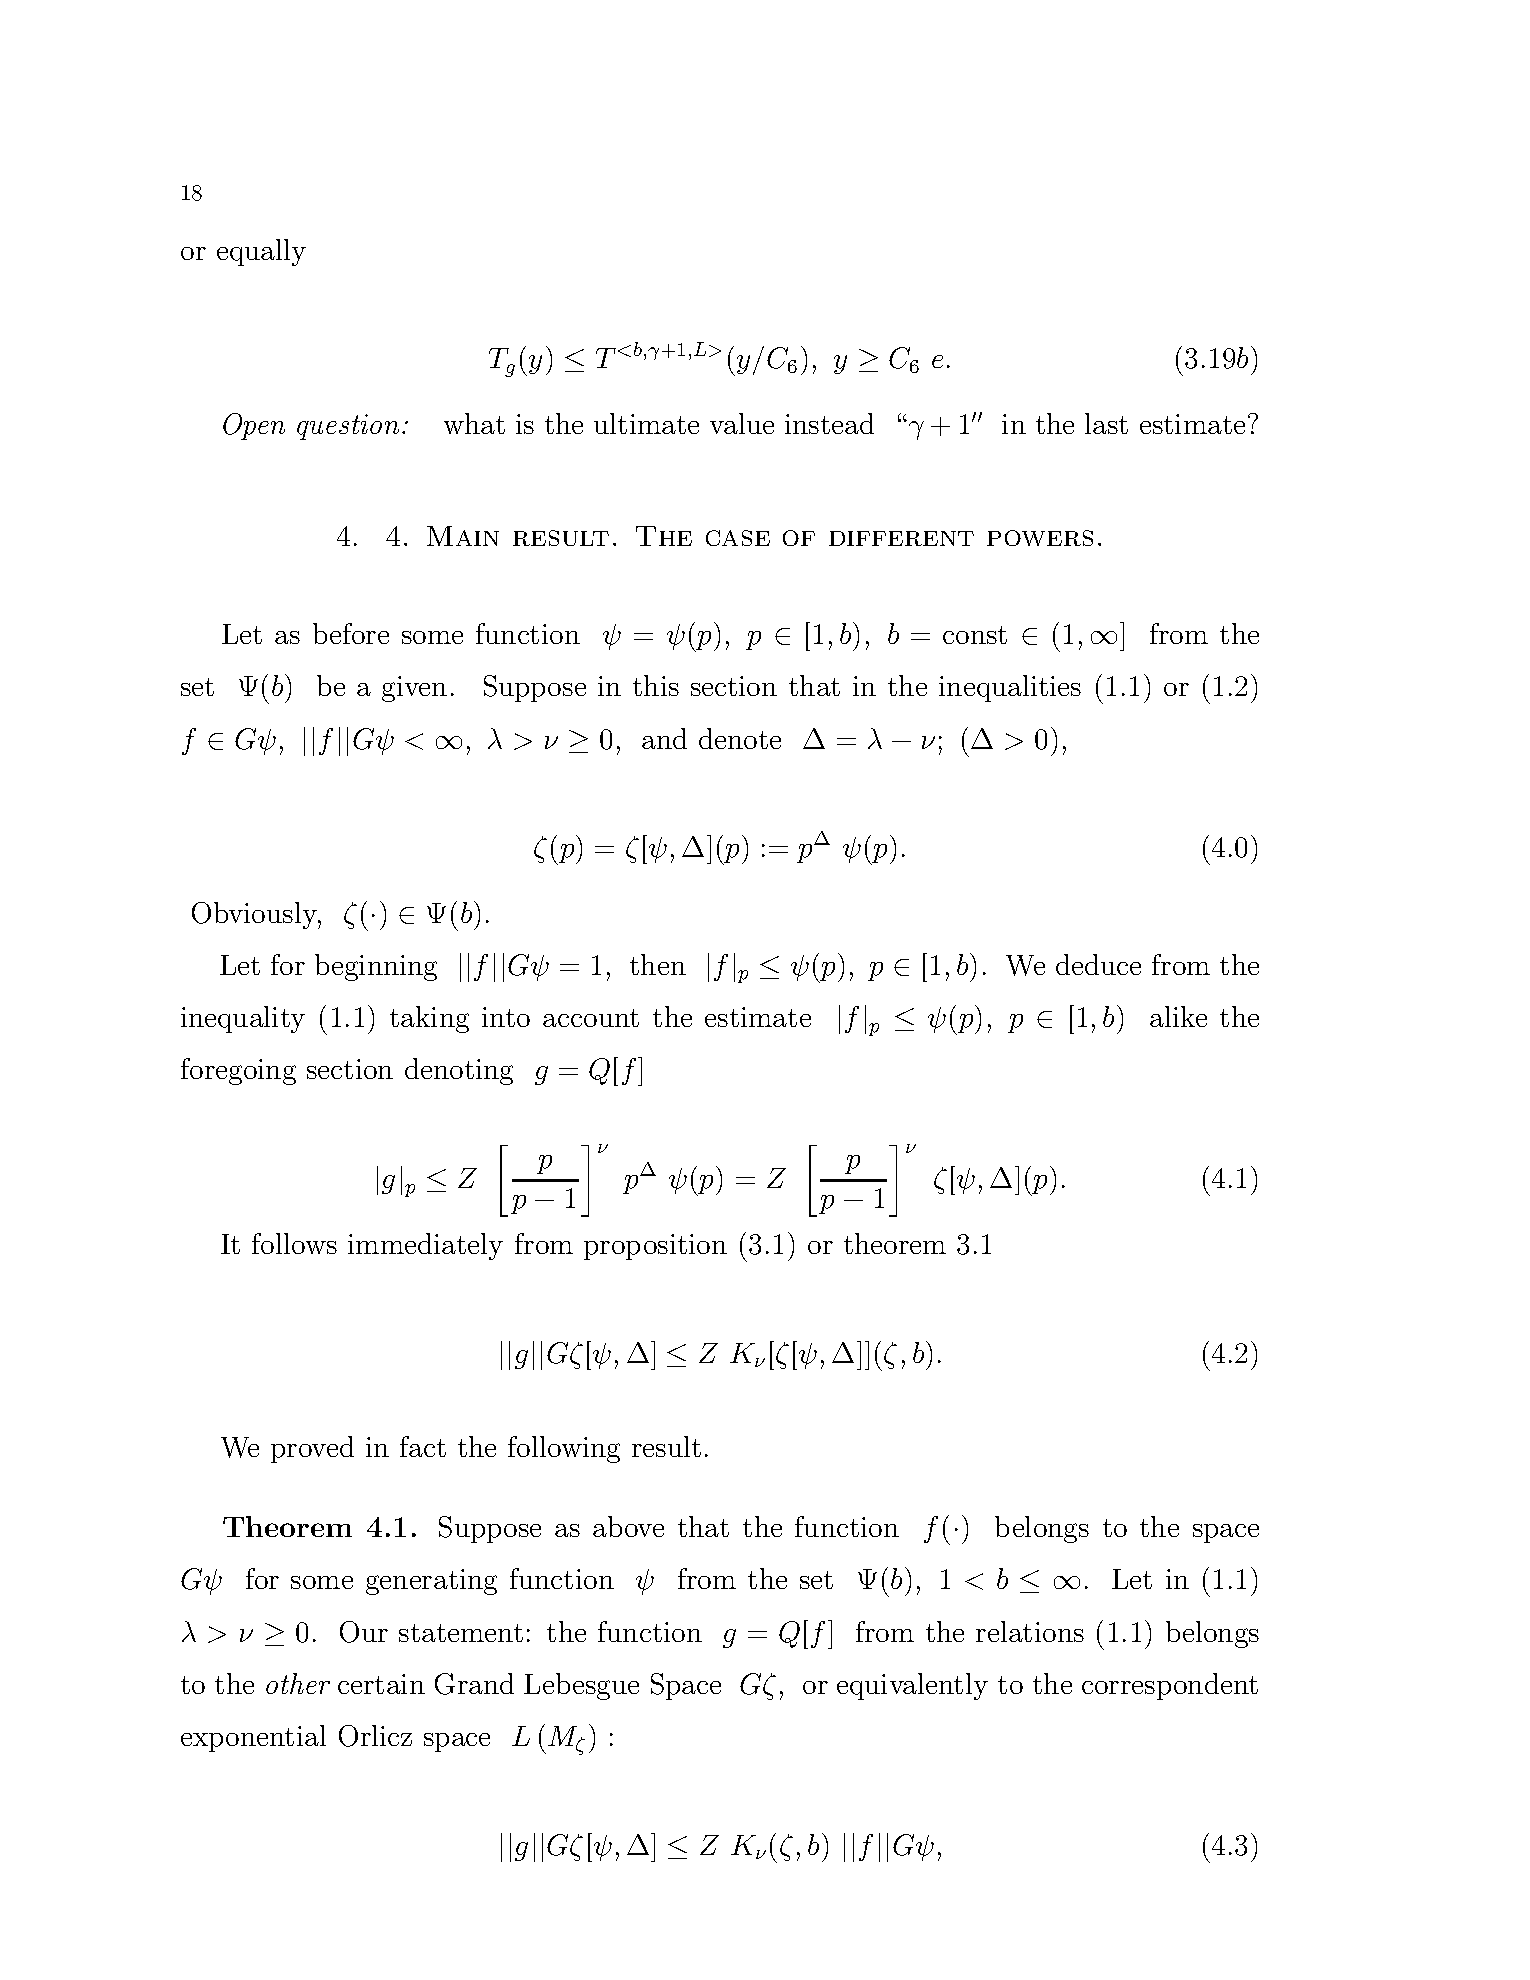
\includegraphics[width=0.94\textwidth]{figures/open_problem_crop_page18.png}
\caption{Source paper, p.~18: (3.19b) and the open question.}
\end{figure}

\section{Answer and proof intuition}

The exponent is \(\gamma+1\).  A moment estimate alone suggests the extra
logarithm, but does not prove it is genuinely attained.  The key is to make it
attained on sparse scales.

On block \(n\), put \(N_n\) equal-mass input atoms at successively smaller
heights.  Their \(b\)-th powers are proportional to \(1/k\).  A norm-one
functional on \(\ell^b_{N_n}\) sends this particular input vector to its full
\(\ell^b\)-norm on one output atom of the same mass.  Since
\(\sum_{k\le N_n}1/k\sim\log N_n\), the output height gains exactly one
logarithm in its \(b\)-th power.  Hölder's inequality shows that the resulting
block operator is contractive not only on \(L^b\), but simultaneously on all
\(L^p\), \(1\le p\le b\).  Rapid separation of the blocks prevents their
input tails from interfering, while the output atoms witness sharpness along
a sequence.

\section{Formal sharpness theorem}

For a measurable random variable \(h\), write
\(\Tp h(y)=\Pp(|h|>y)\).

\begin{theorem}[sharpness of (3.19)]\label{thm:sharp}
Let \(b>1\), \(\gamma>-1\), and let \(L:(0,\infty)\to(0,\infty)\) be
continuous and slowly varying at infinity.  There are a probability space,
a nonnegative measurable function \(f\), and a positive linear operator \(Q\)
such that
\begin{enumerate}
\item \(\|Qh\|_p\le \|h\|_p\) for every \(1\le p\le b\);
\item after a fixed scalar normalization of \(f\),
\[
 \Tp f(y)\le y^{-b}(\log y)^\gamma L(\log y),\qquad y\ge e;
\]
\item for \(g=Qf\) and every \(\beta<\gamma+1\),
\[
 \limsup_{y\to\infty}
 \frac{\Tp g(y)}{y^{-b}(\log y)^\beta L(\log y)}=\infty.
\]
More precisely, for some \(y_n\to\infty\),
\[
 \Tp g(y_n)\gtrsim
 y_n^{-b}(\log y_n)^{\gamma+1}L(\log y_n).
\]
Consequently \(Q\in\mathrm{Type}(\lambda,\lambda)\) with \(Z(Q)=1\) for
every \(\lambda\ge0\), and the exponent \(\gamma+1\) in (3.19) cannot be
replaced by any smaller exponent in the class considered in \cite{OS}.
\end{enumerate}
\end{theorem}

\begin{proof}
Set
\[
 \ellf(t)=t^\gamma L(t),\qquad
 F(x)=x^{-b}\ellf(\log x).
\]
The function \(\ellf\) is regularly varying with index \(\gamma\), while
\(F\) is regularly varying with index \(-b\).  We use only the uniform
convergence and Potter bounds for regularly varying functions
\cite[Theorems 1.2.1 and 1.5.6]{BGT}.

Fix \(0<\alpha<b\).  Choose a sufficiently rapidly increasing sequence
\(R_n\to\infty\), and put
\[
 w_n=e^{-bR_n},\qquad N_n=\lfloor e^{\alpha R_n}\rfloor.
\]
It may be chosen so that
\begin{equation}\label{eq:separation}
 \sum_n(N_n+1)w_n<1,qquad
 \sum_{m>n}N_mw_m\le w_n,
\end{equation}
and so that every height in block \(n+1\) is larger than every height in
block \(n\).  Indeed, \(N_nw_n\asymp e^{-(b-\alpha)R_n}\), whereas the
smallest height introduced below grows like
\(e^{(b-\alpha)R_n/b}\) up to a subexponential factor.  Thus both requirements
follow recursively by taking \(R_{n+1}\) large enough.

Let \(c_0>0\) be fixed and define, for \(1\le k\le N_n\),
\begin{equation}\label{eq:zdef}
 z_{n,k}^b=\frac{c_0\ellf(R_n)}{k w_n}.
\end{equation}
These heights decrease with \(k\).  Uniformly in \(k\le N_n\),
\[
 \frac{\log z_{n,k}}{R_n}
 =\frac1b\left(b-\frac{\log k}{R_n}+o(1)\right)
 \in \left[\frac{b-\alpha}{b}+o(1),1+o(1)\right].
\]
The uniform convergence theorem therefore gives constants \(0<c<C<\infty\)
such that, for all large \(n\) and all \(k\le N_n\),
\begin{equation}\label{eq:Fzk}
 c,k w_n\le F(z_{n,k})\le C,k w_n.
\end{equation}

Construct an atomic probability space with input atoms \(A_{n,k}\)
(\(1\le k\le N_n\)) and one output atom \(B_n\), every one of these atoms
having mass \(w_n\).  Add one residual atom carrying the unused mass.  Define
\(f_0(A_{n,k})=z_{n,k}\) and let \(f_0\) vanish on the output and residual
atoms.

We first verify the input tail.  At a level between \(z_{n,k+1}\) and
\(z_{n,k}\), at most \(k w_n\) of block \(n\) lies above the level, and all
later blocks contribute at most \(w_n\) by \eqref{eq:separation}.  Equation
\eqref{eq:Fzk}, the bounded ratio
\(z_{n,k}/z_{n,k+1}=((k+1)/k)^{1/b}\), and Potter's bound for \(F\) show
\[
 \Tp{f_0}(y)\le C_1F(y),\qquad y\ge y_0.
\]
The same Potter bound handles the gaps between successive blocks; choosing
the first block sufficiently far out handles \(e\le y<y_0\).  Finally replace
\(f_0\) by \(f=a f_0\), where \(a>0\) is sufficiently small.  Since \(F\) is
regularly varying with negative index, this fixed dilation absorbs \(C_1\)
and yields
\begin{equation}\label{eq:inputtail}
 \Tp f(y)\le F(y),\qquad y\ge e.
\end{equation}

For each block set
\[
 Y_n=\left(\sum_{k=1}^{N_n}z_{n,k}^b\right)^{1/b},
 \qquad
 a_{n,k}=\frac{z_{n,k}^{,b-1}}{Y_n^{,b-1}}.
\]
Define the positive linear operator \(Q\) by
\[
 Qh(B_n)=\sum_{k=1}^{N_n}a_{n,k}h(A_{n,k}),
 \qquad Qh=0\quad\text{off }\bigcup_n B_n.
\]
If \(b'=b/(b-1)\), then
\[
 \sum_{k=1}^{N_n}a_{n,k}^{b'}=1.
\]
For \(1<p\le b\), one has \(p'\ge b'\), hence
\(\|(a_{n,k})\|_{p'}\le\|(a_{n,k})\|_{b'}=1\).  Hölder's inequality,
followed by summation over the disjoint blocks, gives
\[
 \|Qh\|_p^p
 =\sum_n w_n\left|\sum_k a_{n,k}h(A_{n,k})\right|^p
 \le\sum_{n,k}w_n|h(A_{n,k})|^p
 \le\|h\|_p^p.
\]
The case \(p=1\) follows from \(\max_k a_{n,k}\le1\).  This proves the
simultaneous contraction assertion.

The coefficients were chosen to norm the particular input vector:
\[
 Qf_0(B_n)=\sum_k\frac{z_{n,k}^{b}}{Y_n^{b-1}}=Y_n.
\]
By \eqref{eq:zdef} and the harmonic sum,
\begin{align*}
 Y_n^b
 &=\frac{c_0\ellf(R_n)}{w_n}
   \sum_{k=1}^{N_n}\frac1k\\
 &\asymp w_n^{-1}R_n^{\gamma+1}L(R_n).
\end{align*}
Because \(\log L(R_n)=o(\log R_n)\), this implies
\(\log Y_n=R_n+o(R_n)\).  Slow variation now yields
\begin{equation}\label{eq:outputscale}
 w_n\asymp
 Y_n^{-b}(\log Y_n)^{\gamma+1}L(\log Y_n).
\end{equation}
For \(g=Qf=aQf_0\), the atom \(B_n\) gives
\(\Tp g(aY_n/2)\ge w_n\).  Combining this with
\eqref{eq:outputscale} and fixed-dilation invariance of regular variation,
for every \(\beta<\gamma+1\),
\[
 \frac{\Tp g(aY_n/2)}
 {(aY_n/2)^{-b}(\log(aY_n/2))^\beta L(\log(aY_n/2))}
 \gtrsim (\log Y_n)^{\gamma+1-\beta}\longrightarrow\infty.
\]
This proves all assertions.
\end{proof}

\section{Why this answers the source question}

The paper already proves the upper estimate with exponent \(\gamma+1\).
Theorem~\ref{thm:sharp} shows that every smaller exponent fails, for each
\(b>1\) and \(\gamma>-1\), and even for positive linear contractions.  Such a
contraction satisfies
\[
 \|Qh\|_p\le \|h\|_p
 \le \left(\frac p{p-1}\right)^\lambda\|h\|_p,
 \qquad 1<p<b,
\]
for every \(\lambda\ge0\).  It therefore lies in every equal-power class
\(\mathrm{Type}(\lambda,\lambda)\) used in Section 3 of the source.  The
optimal universal exponent is consequently exactly \(\gamma+1\).

\section{Verification notes}

The proof is entirely analytic.  The accompanying script
\texttt{code/check\_finite\_blocks.py} checks finite blocks for representative
parameters.  It verifies numerically that the coefficient vector has
\(\ell^{b'}\)-norm one, its \(\ell^{p'}\)-norm is at most one for \(p\le b\),
and the output scale contains the harmonic factor.  This is a consistency
check, not part of the proof.  The command
\begin{center}
\texttt{python code/check\_finite\_blocks.py}
\end{center}
was run for \(b=2\), \(\gamma=0.5\), \(L=1\), \(\alpha=0.8\), and
\(R=4,6,8,10,12\).  In every case \(\|a\|_{b'}=1\) to twelve displayed
decimal places and all tested \(\|a\|_{p'}\le1\); the normalized
\(\gamma+1\) output scale stayed between \(0.66\) and \(0.70\), while the
ratio for the smaller test exponent \(\beta=\gamma+0.5\) increased from
\(1.51\) to \(2.56\).

The most important human-review points are:
\begin{enumerate}
\item the uniform use of regular variation in \eqref{eq:Fzk};
\item the tail bookkeeping across rapidly separated blocks;
\item the endpoint norm comparison \(p'\ge b'\), which is what makes the
operator simultaneously contractive for all \(p\le b\).
\end{enumerate}

\section{Novelty check and limitations}

A bounded search was performed on 9 August 2026.  The local run registry,
solution, attempt, and proof-gap indexes were searched for arXiv:1706.07539,
the paper title, and the core tail/exponent terms.  Web searches used the
exact phrase ``what is the ultimate value'', the exact title, and combinations
of ``bounded support'', ``Grand Lebesgue'', ``maximal operator'', and the
\(\gamma+1\) tail exponent.  They surfaced the source paper but no later arXiv
paper or primary-source answer to this exact question.  This is a bounded
novelty check, not a definitive citation survey.

The result identifies the sharp exponent for the broad operator class defined
only through the \(L^p\) estimates in the source.  A narrower class with extra
structure (for example, a particular geometric maximal operator) could obey a
better endpoint tail law; no such narrower claim is made here.

\begin{thebibliography}{9}
\bibitem{OS}
E. Ostrovsky and L. Sirota,
\emph{Maximal and other operators in exponential Orlicz and Grand Lebesgue
Spaces}, arXiv:1706.07539, 2017.

\bibitem{BGT}
N. H. Bingham, C. M. Goldie, and J. L. Teugels,
\emph{Regular Variation}, Encyclopedia of Mathematics and its Applications
27, Cambridge University Press, 1987.
\end{thebibliography}

\end{document}
